%%%%%%%%%%%%%%%%%%%%%%%%%%%%%%%%%%%%%%%%%
% TMESC Dissertation
% LaTeX Template
% Version 0.2 (Aug/2023)
%
% Adapted to MESCC/ISEP (Apr/2023, Aug/2023 & Nov/2023) by
% Luis Miguel Pinho
%
% Based on TMDEI/ISEP style (Dec/2015) by
%  Nuno Pereira (nap@isep.ipp.pt) and
%  Paulo Baltarejo (pbs@isep.ipp.pt)
%
% Based on MastersDoctoralThesis Version 1.2 by Vel (vel@latextemplates.com) and
% Johannes Böttcher, downloaded from (21/11/15):
% http://www.LaTeXTemplates.com
%
% This template is originally based on a template by:
% Steve Gunn (http://users.ecs.soton.ac.uk/srg/softwaretools/document/templates/)
% Sunil Patel (http://www.sunilpatel.co.uk/thesis-template/)
%
% Template license:
% CC BY-NC-SA 3.0 (http://creativecommons.org/licenses/by-nc-sa/3.0/)
%
%%%%%%%%%%%%%%%%%%%%%%%%%%%%%%%%%%%%%%%%%

%----------------------------------------------------------------------------------------
%	PACKAGES AND OTHER DOCUMENT CONFIGURATIONS
%----------------------------------------------------------------------------------------

\documentclass[
11pt, % The default document font size, options: 10pt, 11pt, 12pt
%oneside, % Two side (alternating margins) for binding by default, uncomment to switch to one side (for drafting/reading purposes)
english, % english for English;
singlespacing, % Single line spacing, alternatives: onehalfspacing or doublespacing (for drafting/reading purposes)
%draft, % Uncomment to enable draft mode (no pictures, no links, overfull hboxes indicated)
%nolistspacing, % If the document is onehalfspacing or doublespacing, uncomment this to set spacing in lists to single
liststotoc, % Uncomment to add the list of figures/tables/etc to the table of contents (not recommended)
%toctotoc, % Uncomment to add the main table of contents to the table of contents (not recommended)
parskip, % Add space between paragraphs (recommended)
%nohyperref, % Uncomment to not load the hyperref package (not recommended)
nohyperreflinkcolor, % hyperref links are not colored (comment to color links, for example to produce an electronic-only version)
headsepline, % Uncomment to get a line under the header
]{tmesc-style} % The class file specifying the document structure

\usepackage{tikz} % Required for creating graphics programmatically (can be removed if not used)
%\usetikzlibrary{arrows} % Required for fancy arrows in TiKZ graphics (can be removed if not used)

\usepackage{pgfplots} % Required for drawing high--quality function plots (can be removed if not used)
\pgfplotsset{compat=newest}

%
% Next you have examples of admissable citation styles; we recommend using the authoryear-comp citation style (which resembles Harvard); don't forget to only uncomment one
%

% authoryear-comp: recommended citation style (e.g. (Buendía, 1860), (Buendía 1910, Arcadio 1940))
%\usepackage[style=authoryear-comp,backend=biber]{biblatex} % Bibtex backend with the authoryear-comp citation style (authoryear citations, bibliography ordered alphabetically)

% numeric citation style (e.g. [1], [1-3])
\usepackage[style=numeric-comp,sorting=none,backend=biber]{biblatex} % Bibtex backend with the numeric-comp citation style (numeric citations, bibliography ordered by appearance)

% alphabetic citation style (e.g. [Buendía10], [Buendía10, Arcadio40])
%\usepackage[style=alphabetic,sorting=none,backend=biber]{biblatex} % Bibtex backend with the alphabetic citation style (alphabetic citations, bibliography ordered by appearance)

\usepackage{enumerate}
\usepackage[shortlabels]{enumitem}
\usepackage{hyperref}
\usepackage{rotating}
\addbibresource{mainbibliography.bib} % The filename of the bibliography

\makeglossaries % build the glossary

%----------------------------------------------------------------------------------------
%	THESIS INFORMATION
%----------------------------------------------------------------------------------------

\thesistitle{Variable Pitch System for UAV proprotors} % Your thesis title, this is used in the title, print it elsewhere with \ttitle
\author{Carlos André Pinto Ramos Gonçalves Rijo} % Your name, this is used in the title page, print it elsewhere with \authorname
\supervisor{Ricardo Augusto Rodrigues Da Silva Severino} % Your supervisor's name, this is used in the title page, print it elsewhere with \supname
\cosupervisor{José Renato Santos Machado} % Your co-supervisor's name, this is used in the title page, print it elsewhere with \cosupname (comment, if no co-supervisor)

\keywords{Keyword1, ..., Keyword6} % Please define up to 6 keywords that better describe your work, print it elsewhere with \keywordnames

\thesisdate{Porto, \today} % thesis date,  print it elsewhere with \tdate

\hypersetup{pdftitle=\ttitle} % Set the PDF's title to your title
\hypersetup{pdfauthor=\authorname} % Set the PDF's author to your name
\hypersetup{pdfkeywords=\keywordnames} % Set the PDF's keywords to your keywords

\begin{document}


%----------------------------------------------------------------------------------------
%	FRONT MATTER
%----------------------------------------------------------------------------------------

% Include the frontmatter of your thesis here

% we include the glossary here (frontmatter is included with \input, so this command is as if it was in main.tex)
%All acronyms must be written in this file.
\newacronym{CPU}{CPU}{Central Processing Units}
\newacronym{COTS}{COTS}{Commercial Off-The Shelf}
\newacronym{FPGA}{FPGA}{Field-Programmable Gate Arrays}
\newacronym{GNSS}{GNSS}{Global Navigation Satellite System}
\newacronym{PCB}{PCB}{Pinted Circuit Board}
\newacronym{PWM}{PWM}{Pulse Width Modulation}
\newacronym{OBC}{OBC}{On Board Computer}
\newacronym{uav}{UAV}{Unmanned Aerial Vehicle}
\newacronym{RPM}{RPM}{Revolutions Per Minute}
\newacronym{RTC}{RTC}{Real-Time Clock}
\newacronym{RTOS}{RTOS}{Real-Time Operating System}
\newacronym{SoC}{SoC}{State of Charge}
\newacronym{UVP}{UVP}{Under Voltage Protection}
\newacronym{VTOL}{VTOL}{Vertical Take-Off and Landing}
\newacronym{EEPROM}{EEPROM}{Electrically Erasable Programmable Read-Only Memory}
\newacronym{SRAM}{SRAM}{Static Random Access Memory}
\newacronym{DRAM}{DRAM}{Dynamic Random Access Memory}
\newacronym{SD}{SD}{Secure Digital}
\newacronym{FRAM}{FRAM}{Ferroelectric Random Access Memory}
\newacronym{RAM}{RAM}{Random Access Memory}
\newacronym{SLC}{SLC}{Single-Level Cell}
\newacronym{MLC}{MLC}{Multi-Level Cell}
\newacronym{TLC}{TLC}{Triple-Level Cell}
\newacronym{eMMC}{eMMC}{embedded MultiMedia Card}
\newacronym{SSD}{SSD}{Solid State Drives}
\newacronym{HDD}{HDD}{Hard Disk Drives}
\newacronym{Li-ion}{Li-ion}{Lithium-ion}
\newacronym{Li-Po}{Li-Po}{Lithium Polymer}
\newacronym{NiMH}{NiMH}{Nickel–Metal Hydride}
\newacronym{NiCd}{NiCd}{Nickel-Cadmium}
\newacronym{ROS}{ROS}{Robot Operating System}
\newacronym{DDS}{DDS}{Data Distribution Service}
\newacronym{I2C}{I2C}{Inter-Integrated Circuit}
\newacronym{SPI}{SPI}{Serial Peripheral Interface}
\newacronym{UART}{UART}{Universal Asynchronous Receiver-Transmitter}
\newacronym{BLE}{BLE}{Bluetooth Low Energy}
\newacronym{TLS}{TLS}{Transport Layer Security}
\newacronym{Wifi}{Wifi}{Wireless Fidelity}
\newacronym{FIFO}{FIFO}{First In First Out}
\newacronym{USB}{USB}{Universal Serial Bus}
\newacronym{CAN}{CAN}{Controller Area Network}
\newacronym{RFID}{RFID}{Radio Frequency Identification}
\newacronym{NFC}{NFC}{Near Field Communication}
\newacronym{HDL}{HDL}{Hardware Description Languages}
\newacronym{ADC}{ADC}{Analog Digital Converter}
\newacronym{IoT}{IoT}{Internet of Things}
\newacronym{IEEE}{IEEE}{Institute of Electrical and Electronics Engineers}
\newacronym{LoRaWAN}{LoRaWAN}{Long Range Wide Area Network}


\frontmatter % Use roman page numbering style (i, ii, iii, iv...) for the pre-content pages

\pagestyle{plain} % Default to the plain heading style until the thesis style is called for the body content

%----------------------------------------------------------------------------------------
%	TITLE PAGE
%----------------------------------------------------------------------------------------

\maketitlepage


%----------------------------------------------------------------------------------------
%	ABSTRACT PAGE
%----------------------------------------------------------------------------------------

\begin{abstract}

% here you put the abstract in the main language of the work.

TODO - abstract up to 200 words

\end{abstract}

\begin{abstractotherlanguage}
% here you put the abstract in the "other language": English, if the work is written in Portuguese; Portuguese, if the work is written in English.

TODO - abstract up to 1000 words ???
%\footnote{Alterar a língua requer apagar alguns ficheiros temporários}.
\end{abstractotherlanguage}


%----------------------------------------------------------------------------------------
%	LIST OF CONTENTS/FIGURES/TABLES PAGES
%----------------------------------------------------------------------------------------

\tableofcontents % Prints the main table of contents

\listoffigures % Prints the list of figures

\listoftables % Prints the list of tables

\listofalgorithms % Prints the list of algorithms
\addchaptertocentry{\listalgorithmname}


% \renewcommand{\lstlistlistingname}{List of Source Code}

% \lstlistoflistings % Prints the list of listings (programming language source code)
% \addchaptertocentry{\lstlistlistingname}


%----------------------------------------------------------------------------------------
%	ABBREVIATIONS
%----------------------------------------------------------------------------------------
\begin{abbreviations}{ll} % Include a list of abbreviations (a table of two columns)
\textbf{FC} & \textbf{F}light \textbf{C}ontroller\\
\textbf{FPP} & \textbf{F}ixed \textbf{P}itch \textbf{P}roprotor\\
\textbf{MDU} & \textbf{M}ain \textbf{D}evice \textbf{U}nit\\
\textbf{SDU} & \textbf{S}econdary \textbf{D}evice \textbf{U}nit\\
\textbf{VPP} & \textbf{V}ariable \textbf{P}itch \textbf{P}roprotor\\

\end{abbreviations}

%----------------------------------------------------------------------------------------
%	SYMBOLS
%----------------------------------------------------------------------------------------

% \begin{symbols}{lll} % Include a list of Symbols (a three column table)

% % [Note: Although acronyms and symbols are defined in this section, they should also be defined at least the first time used in the dissertation body.]

% $a$ & distance & \si{\meter} \\
% $P$ & power & \si{\watt} (\si{\joule\per\second}) \\
% %Symbol & Name & Unit \\

% \addlinespace % Gap to separate the Roman symbols from the Greek

% $\omega$ & angular frequency & \si{\radian} \\

% \end{symbols}



%----------------------------------------------------------------------------------------
%	ACRONYMS
%----------------------------------------------------------------------------------------

\newcommand{\listacronymname}{List of Acronyms}

%Use GLS
\glsresetall
\printglossary[title=\listacronymname,type=\acronymtype,style=long]

%----------------------------------------------------------------------------------------
%	DONE
%----------------------------------------------------------------------------------------

\mainmatter % Begin numeric (1,2,3...) page numbering
\pagestyle{thesis} % Return the page headers back to the "thesis" style


%----------------------------------------------------------------------------------------
%	MAIN BODY
%----------------------------------------------------------------------------------------

% Include the chapters of the thesis as separate folders for each chapter
% Uncomment the lines as you write the chapters

\chapter{Introduction}
\label{chap:Chapter1}
%-------------------------------------------------------------------------------%
\glspl{uav} have witnessed a surge in popularity and research attention. 
They have become indispensable in various applications, ranging from surveillance to reconnaissance, due to their versatility and efficiency in various applications \cite{uav1}. 

This growing interest is evident in the numerous review papers exploring different aspects of \gls{uav} development, ranging from open-source hardware and software utilization \cite{uav2}, \cite{uav3},\cite{uav4}, frame design and optimization \cite{uav5}, \cite{uav6}, control systems, including both conventional and modern communication modalities such as 5G networks \cite{uav7}, \cite{uav8}, \cite{uav10}, \cite{uav11}, to efficient power management strategies, and alternative energy sources to extend \gls{uav} battery life \cite{uav15}.\\

Nowadays, most \gls{VTOL} \glspl{uav}, rely on proprotors with fixed pitch systems because of their simplicity and lack of better \gls{COTS} reliable and efficient solutions but they impose limitations on the achievable flight performance \cite{FPP1}.
Thrust generation is confined to a single direction, hindering the \gls{uav}'s ability to produce upward thrust relative to the vehicle body.
Additionally, the control bandwidth is restricted by the inertia of the motors and proprotors, constraining the \gls{uav}'s agility and maneuverability \cite{FPP1}.\\
As described in recent studies \cite{FPP1}, these limitations become more pronounced as \gls{uav} size increases, impacting stability and control. 
Larger \glspl{uav} face challenges as the need for larger motors with higher inertia compromises rapid control through \gls{RPM} adjustments alone.\\

The development of Variable Pitch Proprotor (VPP) systems plays a crucial role in overcoming the limitations of traditional \gls{uav} designs, such as those with fixed pitch proprotors \cite{VPP1}, \cite{FPP1}.
Several detailed descriptions of quadrotors, for instance, modeling and dynamics have been published \cite{FPP2}, \cite{FPP3}, \cite{FPP4}, \cite{FPP5}, emphasizing the need for dynamic control mechanisms.\\
The use of VPP systems, especially in \gls{VTOL} \glspl{uav}, addresses challenges related to control instabilities and energy efficiency \cite{VPP1}.\\
The incorporation of variable-pitch proprotors provides the necessary flexibility to enhance stability and enable larger \glspl{uav} to perform sophisticated maneuvers, overcoming the constraints inherent in fixed-pitch designs \cite{VPP1}, \cite{FPP1}.

TODO: MORE INFO

\href{https://www.youtube.com/watch?v=MpsBOQOUB-4}{\textit{VPP Video}}

\section{Problem Analyses}
The utilization of fixed-pitch propellers in \glspl{uav} presents a set of limitations that significantly impact aircraft performance and efficiency.
These issues are evident in various phases of flight, including hover and forward flight, and have repercussions for the \gls{uav}.

TODO: MORE INFO

\subsection{Maneuverability and Response}
Fixed-pitch propellers inherently constrain \glspl{uav} from adjusting the pitch angle during flight \cite{FPP1}. 
This limitation results in compromised maneuverability and response, restricting the range of aerobatic maneuvers that a \gls{uav} can execute \cite{FPP1}. 
Additionally, the inability to change the pitch angle impedes the optimization of lift, landing, and thrust during flight, leading to sub-optimal performance in various operational scenarios \cite{FPP1}.

TODO: MORE INFO

\subsection{Power Consumption}
With fixed-pitch propellers, the power consumption will be higher.
Without the ability to adjust the propeller angle, \glspl{uav} may be forced to operate at higher \gls{RPM}s to compensate for this lack of adjustment \cite{FPP1}.
This higher power consumption not only affects the efficiency of the \gls{uav} but also has implications for its endurance, limiting the time the vehicle can remain airborne.\\

TODO: MORE INFO

\section{Motivation}
TODO: MORE INFO

\section{Objectives}
TODO: MORE INFO
\chapter{State of the Art} 
\label{chap:Chapter2}
%-------------------------------------------------------------------------------%
\section{UAV}
\subsection{VTOL}
\subsection{Fixed Pitch Proprotors}
\subsection{Variable Pitch Proprotors}
Historically, early aviation pioneers experimented with propellers that could only be adjusted on the ground.
The first automatic variable pitch air screw was patented by L. E. Baines in 1919.
The Gloster Hele-Shaw Beacham variable pitch propeller, developed in 1928, demonstrated practical controllable pitch capabilities.
Over time, various designs and mechanisms, including hydraulic and pneumatic systems, were explored and refined.
The development of constant-speed propellers marked a significant advancement in aviation technology, offering improved efficiency and performance \cite{VPP2}.\\

A significant advantage of variable-pitch propellers is their ability to adapt to varying airspeeds. 
When an aircraft is stationary or moving slowly, the propeller blades can be set to a low angle of attack to reduce drag. As the aircraft gains speed, the pitch is increased to maintain optimal performance. 
This adaptability ensures efficient operation across a range of flight conditions.

The primary purpose of variable pitch propellers is to maintain the optimal angle of attack relative to the changing wind vector as the aircraft accelerates.
Traditional fixed-pitch propellers face efficiency challenges in various flight conditions.
Adjustable blade angles address this issue, allowing for improved efficiency during takeoff, climb, and cruise.\cite{VPP3}.\\

Variable-pitch systems can adjust blade pitch to maintain a selected \gls{RPM} enhancing overall performance, especially at high altitudes, by allowing the rotor to operate in its most economical speed range\cite{VPP2},\cite{VPP3}.\\

Three methods change the pitch: Hydraulic, Centrifugal, and Electromechanical control \cite{VPP2}.\\
\subsubsection{Hydraulic Method}
This system involves the use of engine oil pressure to control the pitch-changing mechanism and consists of a pump, control valves, and cylinders that actuate the movement of the propeller blades.
In an aircraft without a variable-pitch proprotor system, the pilot uses hydraulics to manually control the pitch of the propeller blades \cite{VPP2}.\\

Hydraulic systems provide a precise means of adjusting the propeller pitch, allowing efficient performance under different flight conditions, and contributing to the overall safety and reliability of the system.\\

But Hydraulic systems add complexity and weight to the overall aircraft system. 
More components means more elements could potentially fail or require maintenance. 
There is also the risk of fluid leakage or fluid contamination that may lead to a reduction in hydraulic pressure, potentially affecting the pitch control mechanism.
Hydraulic systems may have a slow response time due to the time it takes for hydraulic pressure changes to propagate through the system which might be a concern in situations where rapid adjustments are required.\cite{VPP2}

\subsubsection{Centrifugal Method}
In the centrifugal systems, centrifugal weights can be attached directly to the propellers.
An eccentric weight is placed near or in the spinner and secured with a spring and, when the propeller reaches a certain \gls{RPM}, centrifugal force swings the weights outward, driving a mechanism that twists the propeller to a steeper pitch. 
As the propeller slows down, the \gls{RPM} drops and the spring pushes the weight back, readjusting the propeller pitch to a shallower pitch.

As advantages, centrifugal systems are simpler compared to hydraulic systems since they involve fewer components.
The reliance on mechanical components driven by centrifugal force can enhance reliability because there are fewer points of failure.
There is no need to use external power sources, such as an engine-driven pump.
Also, centrifugal systems can operate automatically without direct pilot intervention.
The system responds to changes in rotational speed without the need for continuous manual control.

However, centrifugal systems may provide less precise pitch control than more advanced hydraulic or electronic systems. This limitation can affect the ability to finely tune the propeller for optimal performance.
The response time of centrifugal systems may be slower compared to more sophisticated systems. This limitation could be a factor in situations where rapid adjustments to the propeller pitch are necessary.\cite{VPP2}

\subsubsection{Electromechanical Method}
These systems involve electric motors and mechanical linkages to control the pitch of the propeller blades.\\

Electromechanical methods provide precise control over the pitch of the propeller blades, can offer rapid response times to changes in flight conditions, are often versatile, and can be adapted for various aircraft configurations.
Compared to certain hydraulic systems, electromechanical systems might require less maintenance.
They often have fewer components prone to wear and can be more straightforward to service.\\

As disadvantages, electromechanical systems, including motors and associated components, can add weight to the aircraft, require electrical power to operate, and are more complex than purely mechanical systems, increasing the chance of failures.\cite{VPP2}
%-------------------------------------------------------------------------------%

\section{Control System}
\subsection{Flight Controller}
\subsection{On Board Computer}
An \gls{OBC} is a device capable of managing and/or controlling various functions such as:
\begin{itemize}
    \item It can manage overall system operation.
    \item Implement safety mechanisms and respond to abnormal conditions.
    \item Execute algorithms and computations required for the system's functionality.
    \item Interface with external devices, sensors, actuators, or other embedded systems.
    \item Implement communication protocols for data exchange.
    \item Manage data storage and retrieval.
    \item Implement power-saving modes when appropriate.
    \item Manage and control peripherals such as communication interfaces, timers, and interrupt controllers.
\end{itemize}

There are, mainly, three types of control units: Microcontrollers, Microprocessors, and \glspl{FPGA}.\\
Microcontrollers are integrated circuits that contain a processor core, memory, and programmable input/output peripherals.
They are compact and cost-effective, have low power consumption, are designed for specific tasks, making them suitable for embedded systems, and often include integrated peripherals like timers, communication interfaces, and ADC.\\
However, microcontrollers have more limited processing power compared to microprocessors and are less flexible for general-purpose computing.\\

Microprocessors or \glspl{CPU} focus on processing tasks and rely on external components for additional functionalities.
As an advantage, they have high processing power (suitable for general-purpose computing), can run complex operating systems, and have greater flexibility in application design.\\
However, microprocessors have higher power consumption, may require additional components for specific applications, and have a larger form factor compared to microcontrollers.\\

\glspl{FPGA} are integrated circuits that can be configured after manufacturing, allowing for custom digital logic circuits. 
They are customizable for specific applications, have parallel processing capabilities, and can be reprogrammed for different tasks.\\
But, they have a higher cost (compared to microcontrollers and microprocessors), have higher power consumption (compared to microcontrollers), and have a steeper learning curve for programming and design.\\
%-------------------------------------------------------------------------------%

\section{Power Management System}
\subsection{Power Distribution}
\subsection{Battery Module}
\subsection{Battery Protection}
%-------------------------------------------------------------------------------%

\section{External Memory and Storage Units}
%-------------------------------------------------------------------------------%

\section{Servo Motors}
\subsection{PWM Generator}
%-------------------------------------------------------------------------------%

\section{Mechanical Switch}
%-------------------------------------------------------------------------------%


\chapter{Technologies}
\label{chap:Chapter3}
%-------------------------------------------------------------------------------%

\section{Battery Module}

Batteries are a critical component in portable embedded systems, providing the necessary energy for the system to work properly.

This way, the battery technology selection must be carefully made to optimize the system performance, \cite{BATT3}.
Different battery chemistries offer varying energy densities, voltages, sizes, weights, cycle lives and costs.

In table \ref{tab:battery_comparison} it is possible to compare the most common battery technologies.

\begin{table}[H]
    \centering
    \resizebox{\textwidth}{!}{
        \begin{tabular}{lccccc}
            \hline
            \textbf{Technology} & \begin{tabular}[c]{@{}c@{}}\textbf{Energy}\\ \textbf{Density}\end{tabular} & \textbf{Voltage} & \textbf{Size/Weight} & \textbf{Cycle Life} & \textbf{Cost} \\ \hline
            \textbf{Li-ion}     & High                                                                       & 3.7V             & Compact/Light        & Good                & Moderate      \\
            \textbf{Li-Po}      & High                                                                       & 3.7V             & Flexible/Light       & Good                & Moderate      \\
            \textbf{NiMH}       & Moderate                                                                   & 1.2V             & Bulky/Heavy          & Moderate            & Moderate      \\
            \textbf{NiCd}       & Moderate                                                                   & 1.2V             & Bulky/Heavy          & Good                & Moderate      \\
            \textbf{Lead-Acid}  & Low                                                                        & 2V (6V, 12V)     & Bulky/Heavy          & Moderate            & Low           \\
            \textbf{Alkaline}   & Moderate                                                                   & 1.5V             & Standard Cylindrical & Poor                & Moderate      \\
        \end{tabular}%
    }
    \caption{Comparison of Battery Technologies}
    \label{tab:battery_comparison}
\end{table}

\gls{Li-ion} and \gls{Li-Po} batteries, shown in figures \ref{fig:18650} and \ref{fig:lipo}, can offer high energy density, rechargeability and moderate costs that make them suitable for portable devices, \cite{BATT7}.
These batteries stand out as a prevalent choice for embedded systems.
\begin{figure}[H]
    \centering
    \begin{minipage}{.5\textwidth}
        \centering
        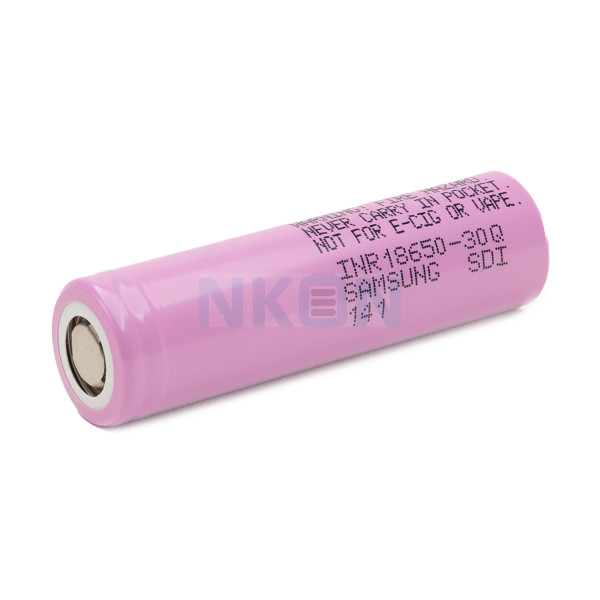
\includegraphics[width=.5\linewidth]{ch3/assets/18650.jpg}
        \captionof{figure}{\gls{Li-ion} battery example \cite{18650}}
        \label{fig:18650}
    \end{minipage}%
    \begin{minipage}{.5\textwidth}
        \centering
        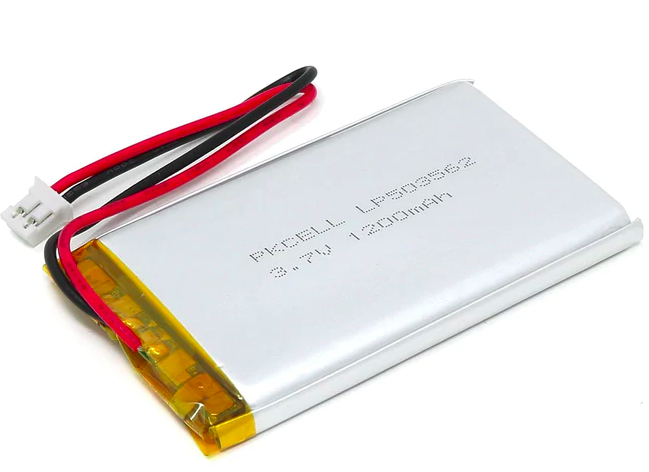
\includegraphics[width=.5\linewidth]{ch3/assets/lipo.png}
        \captionof{figure}{\gls{Li-Po} battery example \cite{lipo}}
        \label{fig:lipo}
    \end{minipage}
\end{figure}

\gls{NiMH} and \gls{NiCd} batteries (figures \ref{fig:nimh} and \ref{fig:nicd} respectably) can provide moderate energy density, rechargeability and moderate costs, but they can be heavier and \gls{NiCd} batteries have a \textit{memory effect} concern (where the battery, falsely, indicates full charge despite being only partially charged).
\begin{figure}[H]
    \centering
    \begin{minipage}{.5\textwidth}
        \centering
        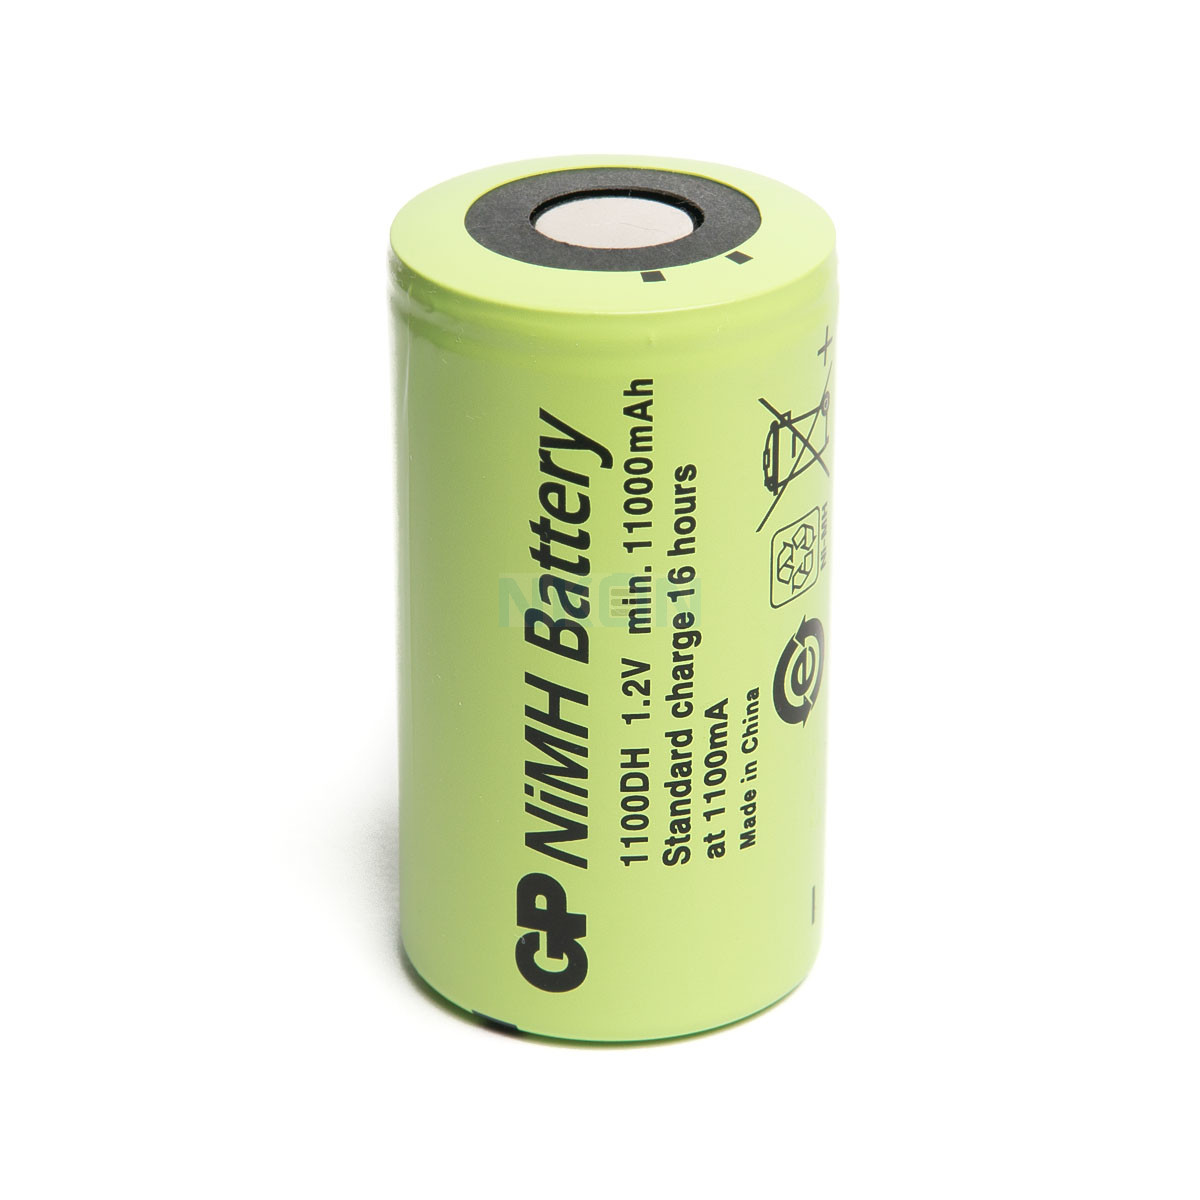
\includegraphics[width=.5\linewidth]{ch3/assets/nimh.jpg}
        \captionof{figure}{\gls{NiMH} battery example \cite{nimh}}
        \label{fig:NiMH}
    \end{minipage}%
    \begin{minipage}{.5\textwidth}
        \centering
        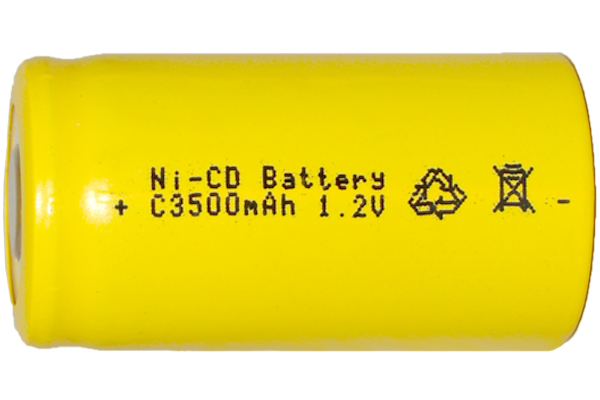
\includegraphics[width=.5\linewidth]{ch3/assets/nicd.jpg}
        \captionof{figure}{\gls{NiCd} battery example \cite{nicd}}
        \label{fig:NiCd}
    \end{minipage}
\end{figure}

Lead-Acid batteries can be rechargeable and cost-effective but heavier and larger and with low energy density.
These batteries are suitable for less portable applications, \cite{BATT3} as it is possible to see in figure \ref{fig:lead}.
\begin{figure}[H]
    \centering
    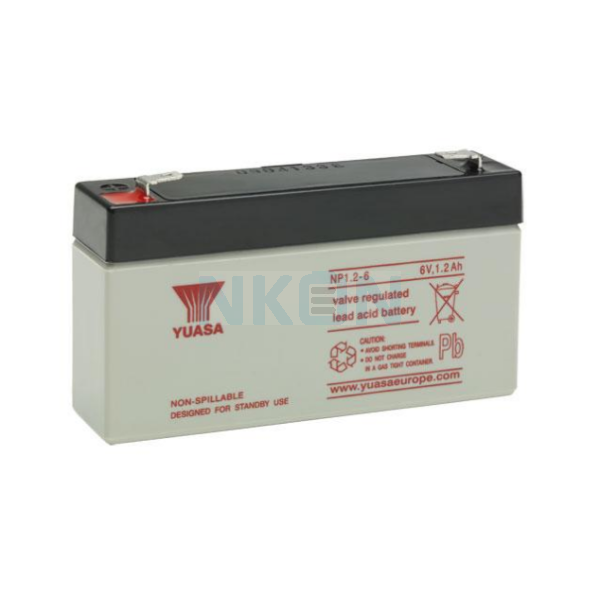
\includegraphics[scale=0.4]{ch3/assets/lead.png}
    \caption{Lead-Acid battery example \cite{lead}}
    \label{fig:lead}
\end{figure}


Alkaline batteries in figure \ref{fig:alkaline} are cost-effective but most of them are non-rechargeable, have a standard cylindrical format and have moderate energy density \cite{BATT3}.
\begin{figure}[H]
    \centering
    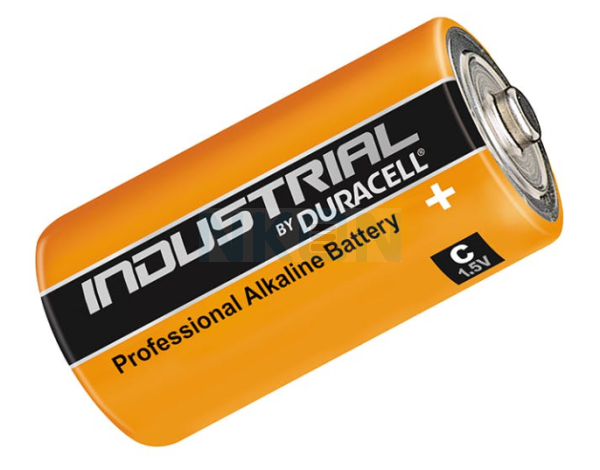
\includegraphics[scale=0.3]{ch3/assets/alkaline.png}
    \caption{Alkaline battery example \cite{alkaline}}
    \label{fig:alkaline}
\end{figure}


%-------------------------------------------------------------------------------%

\section{External Memory and Storage Units}

Memory units can be classified as volatile memory and as non-volatile memory \cite{mem3}.

Volatile storage, like for example \gls{RAM} provides fast read and write speeds and is used for storing variables and managing application stacks.
However, they require constant power to retain data, making them unsuitable for applications with strict power constraints, and have lower memory capacity \cite{mem8}.

Non-volatile storages are suitable for applications requiring frequent data read and write operations and have the capability of being electrically erased and reprogrammed.
They have long-term data retention and low power consumption but have slow access speed compared to volatile storage \cite{mem8}.
These characteristics make non-volatile storages useful for storing configuration parameters and critical data that need to be retained during power cycles.

Often, in embedded systems, the system must be able to store data not only internally (main memory) but also externally (external memory).
External memory units are normally used to expand storage capacity, store data and logs, facilitate data transfer, and backup critical information \cite{mem3}.

Since non-volatile storage can keep the data stored even when they are not powered, these storages are very common in embedded systems \cite{mem1}.

\gls{SD} card, with its multiple formats and sizes, has moderate access speed and can keep data for a long term but it depends on the type (\gls{SLC}, \gls{MLC} and \gls{TLC}).
Typically, the capacity ranges from a few megabytes to multiple terabytes, offering multiple choices for different use cases \cite{mem11}, \cite{mem9}.
However, the moderate power consumption and overall cost can, sometimes, be a setback to the system.

\gls{EEPROM}, commonly used for storing small amounts of data, has fast access speed and a moderate overall cost.
Has long-term data retention and low power consumption but offers lower capacities (in the range of kilobytes to megabytes) making it only suitable for small data storage \cite{mem8}, \cite{mem11}.

\gls{FRAM} combines the benefits of \gls{RAM} and \gls{EEPROM} and can be suitable for applications requiring fast and non-volatile memory.
Has very fast access speed, long-term data retention, low capacity (in the range of kilobytes to megabytes), and very low power consumption.
But has a relatively higher overall cost compared to other technologies \cite{mem8}, \cite{mem11}.

As for \gls{eMMC}, normally found in smartphones, tablets, and other embedded systems, is characterized by its fast access speed, long-term data retention and high capacity (with ranges from megabytes to terabytes).
Like \gls{SD} cards it has moderate power consumption and moderate to high overall cost \cite{mem11}.

\gls{HDD} and \gls{SSD} memory units can have fast access speed, long-term data retention and high capacity (in the range of gigabytes to terabytes).
But, in comparison to other memory units, it has a bigger size, higher power consumption and higher overall cost.
These units are normally used as primary storage in computers and laptops for improved performance, \cite{mem10}.

Table \ref{tab:memory_comparison} compares the described technologies in their access speed, overall cost, data retention, capacity and power consumption.
\begin{table}[H]
    \centering
    \resizebox{\textwidth}{!}{
        \begin{tabular}{lcccccc}
            \hline
                              & \textbf{Access Speed} & \textbf{Overall Cost} & \textbf{Data Retention} & \textbf{Capacity} & \textbf{Power Consumption} \\ \hline
            \textbf{SD Cards} & Moderate              & Moderate              & Long-term               & High              & Moderate                   \\
            \textbf{EEPROM}   & Fast                  & Moderate              & Long-term               & Low               & Low                        \\
            \textbf{FRAM}     & Very Fast             & Relatively Higher     & Long-term               & Low               & Very Low                   \\
            \textbf{eMMC}     & Fast                  & Moderate              & Long-term               & High              & Moderate                   \\
            \textbf{SSD}      & Very Fast             & High                  & Long-term               & Very High         & High                       \\
            \textbf{HDD}      & Moderate              & High                  & Long-term               & very High         & High                       \\\hline
        \end{tabular}
    }\caption{Comparison of External Memory Technologies}
    \label{tab:memory_comparison}
\end{table}

\section{Firmware}
In embedded systems, the choice of programming languages and the use of a \gls{RTOS} in firmware development are critical decisions that can impact the performance, efficiency, and complexity of the embedded system.\\

\subsection{Programming languages}
Even though there are multiple programming languages, normally categorized as low-level or high-level, not all programming languages are optimized to be used in embedded systems.
In this section, an overview and comparison was made on some examples of programming languages.
\subsubsection{C}
\textit{C} programming language has low-level features and is close to the hardware making it efficient and with high performance.

It provides fine-grained control over memory, leading to efficient memory usage but can also lead to potential errors if not handled carefully.
Due to its low-level control and predictable performance, it is often used in real-time systems.

This programming language is generally portable and has a large and active community, with extensive support and numerous libraries, development tools and compilers available.

In terms of safety and reliability, it is a powerful language but lacks some safety features, like in memory management for example.

\textit{C} can have a steeper learning curve, especially for beginners, due to manual memory management and low-level constructs.

\subsubsection{Assembly}
\textit{Assembly} programming language provides direct control over hardware and is highly efficient, and useful for writing low-level code.
It allows developers to directly manage memory, providing fine control over memory footprint.

\textit{Assembly} can be used in real-time systems due to its precise control over hardware, predictable performance and high efficiency.

However, in \textit{Assembly}, there is no safety net or restrictions, this way developers must handle all aspects of safety and reliability manually.
\textit{Assembly} is also highly dependent on the architecture and is not inherently portable, has a niche community, and support is often architecture-specific and relies on specific tools provided by the hardware manufacturer.
The learning curve is steep due to its low-level nature, and development is time-consuming compared to higher-level languages.

\subsubsection{C++}
\textit{C++} programming language is an object-oriented feature that can enhance code organization and reusability and can provide abstraction without sacrificing performance.
It allows both manual and automatic memory management, providing flexibility.
\textit{C++} supports real-time programming, especially with the use of specific frameworks but is not as deterministic as low-level languages.

This programming language benefits from a robust community, with extensive support, it inherits development tools and compilers from \textit{C} and has specific tools for features like object-oriented programming.

C++ introduces features like classes and objects, enhancing code organization and safety compared to C.
However, it still allows low-level operations that may impact reliability.

Since \textit{C++} is similar to \textit{C}, and since it introduces additional concepts, the learning curve can be slightly more complex.
However, its object-oriented features can lead to more maintainable code.

\subsubsection{Rust}
\textit{Rust} programming language, known for its focus on memory safety, is gaining popularity in embedded systems development.
It offers performance similar to \textit{C} and \textit{C++} while providing memory safety features.

\textit{Rust's} was designed with a strong focus on memory safety with an ownership system that helps prevent common memory-related errors without sacrificing performance.
This results in a secure and efficient memory footprint.

As for portability, it aims to be highly portable, with a focus on minimizing platform-specific issues.
With features like Cargo, it simplifies dependency management and project setup.

\textit{Rust} has a growing community and is gaining popularity, with strong support.
However, it can be challenging for beginners due to its ownership system.

\subsubsection{MicroPython}
Efficiency and Performance: MicroPython is designed for microcontrollers and IoT devices, emphasizing efficiency. However, it sacrifices some features of the standard Python to fit within resource constraints.
Memory Footprint: MicroPython aims for a small memory footprint suitable for microcontrollers, enabling its use in resource-constrained environments.
Real-Time Capabilities: MicroPython can be suitable for real-time tasks on microcontrollers, but its capabilities may be limited compared to dedicated real-time operating systems.
Portability: MicroPython is tailored for microcontrollers, enhancing portability within the embedded systems domain.
Community and Support: MicroPython has a growing community focused on supporting embedded systems, with resources specifically tailored to microcontroller development.


Table \ref{tab:programming_languages_comparison} resumes and compares all programming languages described above.
\begin{table}[H]
    \centering
    \resizebox{\textwidth}{!}{
        \begin{tabular}{lcccccc}
            \hline
            \textbf{Topic}             & \textbf{C} & \textbf{C++} & \textbf{Rust} & \textbf{Assembly} & \textbf{MicroPython} \\ \hline
            Efficiency and Performance & High       & High         & High          & Very High         & Moderate             \\
            Memory Footprint           & Low        & Moderate     & Moderate      & Very Low          & Low                  \\
            Real-Time Capabilities     & Limited    & Limited      & Developing    & Yes               & Limited              \\
            Portability                & High       & Moderate     & Moderate      & Low               & High                 \\
            Community and Support      & Large      & Large        & Growing       & Limited           & Growing              \\
            Development Tools          & Abundant   & Abundant     & Growing       & Limited           & Limited              \\
            Safety and Reliability     & Moderate   & Moderate     & High          & Low               & Moderate             \\
            Learning and Development   & Moderate   & Moderate     & Moderate      & Difficult         & Easy                 \\ \hline
        \end{tabular}
    }
    \caption{Comparison of Programming Languages in Embedded Systems}
    \label{tab:programming_languages_comparison}
\end{table}



\subsection{Real-time Operating Systems}
\glspl{RTOS} facilitates multitasking, allowing concurrent execution of multiple tasks, can provide task scheduling, priority management, and inter-process communication and is suitable for systems with real-time requirements.
But this can add overhead, especially in terms of memory footprint, and the learning curve is steeper \cite{RTOS1}.\\
The following \gls{RTOS} examples are open-source, well-documented, compact, and designed for resource-constrained systems, and they support various microcontroller architectures

\subsubsection{FreeRTOS}
\textit{FreeRTOS} is a popular open-source real-time operating system.
micro-ROS has been integrated with FreeRTOS to bring ROS functionality to resource-constrained devices.
DDS implementations like eProsima's Micro XRCE-DDS can be used with FreeRTOS and micro-ROS.

\subsubsection{ChibiOS}
\textit{ChibiOS} is a real-time operating system designed for embedded systems.
It supports micro-ROS, enabling ROS-based communication on microcontroller platforms.
The integration with DDS middleware allows for distributed communication.

\subsubsection{NuttX}
\textit{NuttX} is a real-time operating system with a focus on standards compliance.
It has support for micro-ROS, allowing integration with ROS-based robotic systems.
Micro XRCE-DDS can be used for DDS communication on NuttX.

\subsubsection{Zephyr}
\textit{Zephyr} is a real-time operating system for resource-constrained devices.
It supports micro-ROS, allowing integration with ROS-based robotic systems.
Micro XRCE-DDS is one of the DDS implementations that can be used with Zephyr.

All the \glspl{RTOS} examples, mentioned before, support microROS, an extension of the \gls{ROS}, designed for microcontrollers and embedded systems that can be resource-constrained.
%This makes it possible for the system to participate in \gls{ROS}-based robotic systems with \gls{DDS} as a communication middleware.

\subsection{Comparison}
Programming Languages:
Pros:

Portability: Higher-level languages like C or C++ provide better portability across different hardware platforms.
Productivity: High-level languages can increase developer productivity by abstracting hardware details and providing more expressive syntax.
Code Reusability: Modular code and libraries are more easily reusable, saving time and effort in development.

Cons:

Performance Overhead: High-level languages may introduce performance overhead compared to low-level languages like assembly or C, which can be critical in resource-constrained embedded systems.
Memory Usage: Applications written in high-level languages might consume more memory compared to optimized low-level code.
Limited Control: Developers may have less control over low-level hardware details, which could be essential for certain embedded applications.

Real-Time Operating Systems (RTOS):
Pros:

Deterministic Timing: RTOS provides deterministic timing, crucial for systems where timing constraints are critical.
Task Management: Efficient task scheduling and management enable the execution of multiple tasks simultaneously.
Resource Management: RTOS can effectively manage resources, optimizing CPU and memory usage.

Cons:

Complexity: Integrating an RTOS can introduce complexity, especially for small-scale embedded systems where simplicity is essential.
Overhead: Some RTOS overhead is incurred in terms of both processing time and memory usage.
Learning Curve: Developers may need to invest time in learning and understanding the specific RTOS, adding to the development time.





%-------------------------------------------------------------------------------%

\section{Communication}
TODO: MORE INFO\\
\subsection{Wired}
TODO: MORE INFO\\

\subsection{Wireless}
While researching wireless communication, multiple protocols can be studied. They can, mainly, be separated into two categories: short-range and long-range.
In the context of \glspl{uav}, the focus will be on short-range wireless communication protocols \cite{WCOM1}, \cite{WCOM6}, \cite{WCOM7}.

Short-range protocols offer advantages such as lower power consumption, reduced interference, and efficient data transfer within confined spaces.
Within this category, options like Bluetooth, Wi-Fi, Zigbee, Z-Wave, and LoRa for short distances emerge as noteworthy candidates.
Each of these protocols addresses specific requirements, making them suitable for various aspects of \gls{uav} operations, from intra-component communication to data transfer between the \gls{uav} and ground control \cite{WCOM6}, \cite{WCOM7}.

\begin{itemize}
    \item WiFi (802.11x): Can be used for high-speed data transfer over short ranges. It's suitable when you need to transmit large amounts of data between the \gls{uav} and a ground station.
          \begin{itemize}
              \item Advantages
                    \begin{itemize}
                        \item High Data Rates
                        \item Widespread Standard
                        \item Bi-Directional Communication
                    \end{itemize}
              \item Disadvantages
                    \begin{itemize}
                        \item High Power Consumption
                        \item Interference in 2.4 GHz and 5 GHz bands
                    \end{itemize}
          \end{itemize}

    \item Bluetooth: Common short-range wireless technology with low power consumption. It's suitable for communication between components on a \gls{uav}.
    \item Advantages
          \begin{itemize}
              \item Low Power Consumption
              \item Ubiquity
          \end{itemize}
    \item Disadvantages
          \begin{itemize}
              \item Limited Range
              \item Data Transfer Rates
          \end{itemize}

    \item Zigbee: Low-power, low-data-rate wireless communication technology that is suitable for short-range communication in embedded systems.
    \item Advantages
          \begin{itemize}
              \item Low Power Consumption
              \item Mesh Networking
              \item Low Latency
          \end{itemize}
    \item Disadvantages
          \begin{itemize}
              \item Limited Data Rate
              \item Limited Range
          \end{itemize}

    \item Z-Wave: Low-power wireless communication protocol often used in home automation. It's suitable for control and monitoring applications in \glspl{uav}.
    \item Advantages
          \begin{itemize}
              \item Low Power Consumption
              \item Interference Avoidance
          \end{itemize}
    \item Disadvantages
          \begin{itemize}
              \item Limited Data Rate
              \item Less Common in Non-Home Automation Devices
          \end{itemize}

    \item LoRa (Long Range): While designed for long-range communication, LoRa can also be used in short-range applications. It provides low-power, long-range communication suitable for certain \gls{uav} scenarios.
    \item Advantages
          \begin{itemize}
              \item Long Range
              \item Low Power Consumption
          \end{itemize}
    \item Disadvantages
          \begin{itemize}
              \item Low Data Rates
              \item Unidirectional Communication
          \end{itemize}
\end{itemize}

%-------------------------------------------------------------------------------%

% \section{Power Management System}
% TODO: MORE INFO\\

% \subsection{Power Distribution}
% TODO: MORE INFO\\

% \subsection{Battery Protection}
% \gls{UVP}\\
% Fuse (but a single point of failure)\\
% Reverse polarity Protection\\
% TODO: MORE INFO\\

%-------------------------------------------------------------------------------%
\chapter{Proposed Approach}
\label{chap:Chapter4}
%-------------------------------------------------------------------------------%

\section{Concept}
Fixed-pitch proprotor (FPP) system limitations can be addressed by developing variable-pitch proprotors.
Adjusting the pitch in both flight phases may be more complex and expensive but it offers more adaptability and a great positive impact on the overall propulsion system efficiency, increasing the endurance and range.
The Vehicle will consume less in hover and the cruise speed will be much higher.\\

This way, the proposed solution for this problem is to develop a stand-alone variable-pitch proprotor system that can, in real-time, change the propeller pitch according to each flight phase.

%-------------------------------------------------------------------------------%

\section{Requirements}
It is important to define requirements, for this system, to better understand the fixed-pitch propeller's limitations and to develop the necessary functionalities to achieve a variable-pitch proprotor system.\\
This way, the requirements should align with mechanical, control, communication, integration, and validation specifications.
\begin{itemize}
    \item Mechanical Requirements:
          \begin{itemize}
              \item The system shall be designed to retrofit existing \glspl{uav} or integrate seamlessly into new \gls{uav} designs.
              \item The variable-pitch mechanism shall be lightweight to minimize the impact on overall \gls{uav} weight and balance.
              \item The system shall be able to withstand the operational stresses and environmental conditions encountered during \gls{uav} flights.
          \end{itemize}
    \item Control System Requirements:
          \begin{itemize}
              \item The control system shall enable real-time adjustment of the proprotor pitch during different flight phases.
              \item It shall incorporate failsafe mechanisms to respond to unexpected malfunctions or loss of communication and revert to a fixed-pitch state in case of critical failures.
              \item The system shall provide precise control over the pitch angle, allowing for fine adjustments to optimize performance.
          \end{itemize}
    \item Wireless Communication Requirements:
          \begin{itemize}
              \item The wireless communication system shall be reliable, with minimal latency to ensure quick response times.
              \item It shall operate within designated frequency bands and comply with relevant aviation communication standards.
              \item Security measures shall be implemented to prevent unauthorized access or interference with the control signals.
          \end{itemize}
    \item Integration Requirements:
          \begin{itemize}
              \item The system shall be designed for easy integration with common \gls{uav} autopilot systems.
              \item It shall have compatibility with existing \gls{uav} avionics and navigation systems.
              \item The variable-pitch system shall not interfere with other onboard sensors or communication systems.
          \end{itemize}
    \item Testing and Validation Requirements:
          \begin{itemize}
              \item The system shall undergo rigorous testing under various operational scenarios, including weather conditions and flight profiles.
              \item Validation shall include simulated and real-world flights to assess performance and reliability.
              \item The system shall comply with relevant aviation regulations and standards.
          \end{itemize}
\end{itemize}
%-------------------------------------------------------------------------------%

\section{System Architecture}
As it is possible to see in the proposed implementation of the System Architecture diagram (figure \ref{system_diagram}), the system will be composed of two subsystems: the Main Device Unit (MDU) and (multiple) Secondary Device Unit (SDU).

\begin{figure}[H]
    \centering
    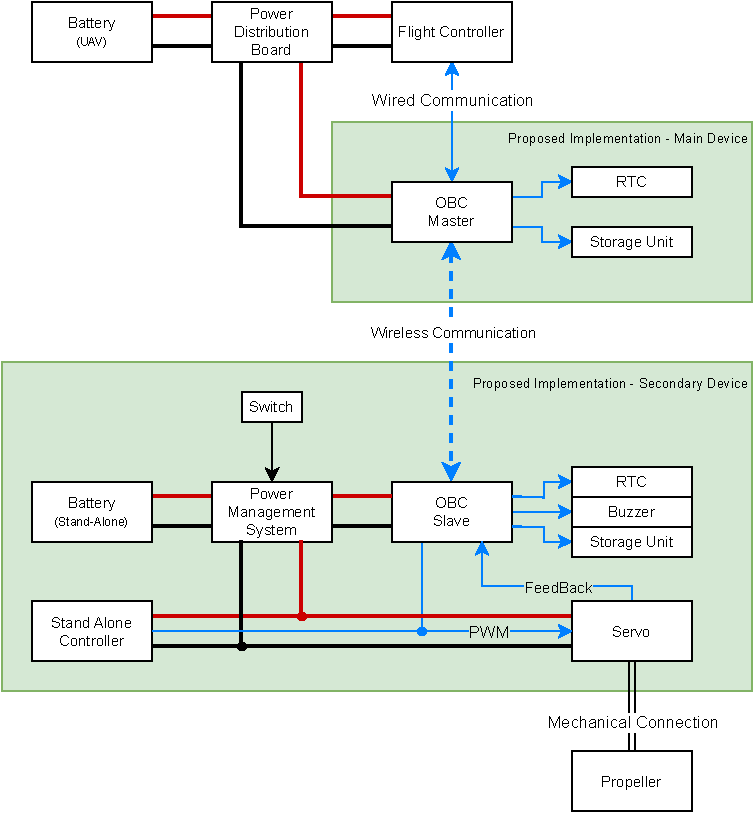
\includegraphics[width=\textwidth,keepaspectratio]{ch4/assets/system_diagram.pdf}
    \caption{Proposed Implementation of System Architecture Diagram}
    \label{system_diagram}
\end{figure}


\subsection{Main Device}
This system will be, mainly, composed of an \gls{OBC}, a \gls{RTC}, a Storage Unit, and a wireless communication module.\\
The MDU will communicate with the Flight Controller and the SDUs by receiving and transmitting information.
With the Flight Controller, through wired communication, the MDU will:
\begin{itemize}
    \item Receive
          \begin{itemize}
              \item Flight Phase message
              \item Maneuver control message
              \item \gls{GNSS} epoch time
              \item Heartbeat signal
          \end{itemize}
    \item Transmit
          \begin{itemize}
              \item Heartbeat signal
              \item System Status message
          \end{itemize}
\end{itemize}

The Flight Phase message and the Maneuver Control message will inform the MDU about the current flight phase and the need to make additional adjustments to the propeller pitch, in case of non-expected maneuvers.
After interpreting the message, the \gls{OBC} will send a control command. This control command will be explained further in this document\\

The \gls{GNSS} epoch time will update the \gls{OBC} date and time (periodically or on startup). With the help of the \gls{RTC}, the MDU system will be able to maintain the date and time even when the \gls{uav} system is powered off.
The \gls{GNSS} epoch time will be helpful when storing system logs (in the Storage Unit) and will help to calculate the latency of the communication between devices.\\

Lastly, the received heartbeat signal will work as a \textit{keep alive} mechanism informing, this way, the \gls{OBC} if the system is powered on.
This will help save power since the \gls{OBC} can shut down when the Flight Controller turns off.\\

The transmitted heartbeat, which also works as a \textit{keep alive} mechanism, will inform the Flight Controller that the MDU is working correctly.
This function will be crucial because if the MDU is not working (powered off or unresponsive) the \gls{uav} system will need to enter a failsafe mode and land, as soon as possible, since it can no longer control the pitch of the blades.\\

Since the MDU is responsible for all the SDUs, it must, periodically, inform the Flight Controller about the overall status of the system, so that, in case of any failure, the Flight Controller may enter in failsafe.\\

With the SDUs, through wireless communication, the MDU will:
\begin{itemize}
    \item Receive
          \begin{itemize}
              \item Heartbeat signal
              \item SDU Status message
          \end{itemize}
    \item Transmit
          \begin{itemize}
              \item Heartbeat signal
              \item Control Command
              \item Epoch Time
          \end{itemize}
\end{itemize}

The received and transmitted heartbeat signals will have the same functionality as explained previously. The MDU and SDUs will inform each other if they are working correctly.\\

The SDU Status message will help the MDU keep track of the status of all Secondary devices. In case of malfunction or if one or more SDUs can't change the propeller pitch, the MDU must be noticed so that it can communicate to the Flight Controller about the failure.\\

The MDU will send a Control Command, containing the desired pitch, to all the SDUs according to the phase of flight message received previously.\\

By sending the epoch time to all the SDUs, it is possible to keep the whole system updated and with the same date and time reference.\\

\subsection{Secondary Device}
This system will be, composed of an \gls{OBC}, a \gls{RTC}, a Storage Unit, a battery (with a power management system), an on/off switch, a buzzer, a stand-alone \gls{PWM} (Pulse Width Modulation) controller, a servo, and a wireless communication module.\\

The on/off switch and the buzzer will work as human-machine interfaces to help the user interact with the system.\\
Since the SDU will be designed to be stand-alone (with a dedicated power supply) the system needs to be powered on manually and the buzzer can notice the user that the system is powering on.\\

The servo, mechanically connected to the propeller, will be responsible for changing the propeller pitch according to the state of flight.
It will be equipped with feedback functionality so that the system can control, more precisely, the pitch and know if the propeller has reached its goal.\\

There will also be implemented a stand-alone \gls{PWM} controller, able to generate a fixed \gls{PWM} signal, to control the servo in case of failure from the \gls{OBC}.
As a failsafe mechanism, if one or more SDUs fail, the \gls{PWM} controller will generate a \gls{PWM} signal fixing the pitch of the propellers to a designated angle.
This action will transform the \gls{uav} system into a fixed-pitch proprotor but will help avoid having a system with a single point of failure that can cause the \gls{uav} to crash and possibly hurt people.\\
%-------------------------------------------------------------------------------%

\section{Timeline}
\chapter{Development Plan}
\label{chap:Chapter5}
%-------------------------------------------------------------------------------%
\section{Research Approach}
%-------------------------------------------------------------------------------%

\section{Evaluation}
%-------------------------------------------------------------------------------%

\section{Timeline}



%----------------------------------------------------------------------------------------
%	BIBLIOGRAPHY
%----------------------------------------------------------------------------------------

\printbibliography[heading=bibintoc]

%----------------------------------------------------------------------------------------
%	THESIS CONTENT - APPENDICES
%----------------------------------------------------------------------------------------

\appendix % Cue to tell LaTeX that the following "chapters" are Appendices

% Include the appendices of the thesis as separate files from the Appendices folder
% Uncomment the lines as you write the Appendices

% Appendix A

\chapter{Main Device Flow Chart - Prepare Task} % Main appendix title

\label{AppendixA}

\begin{figure}[H]
    \centering
    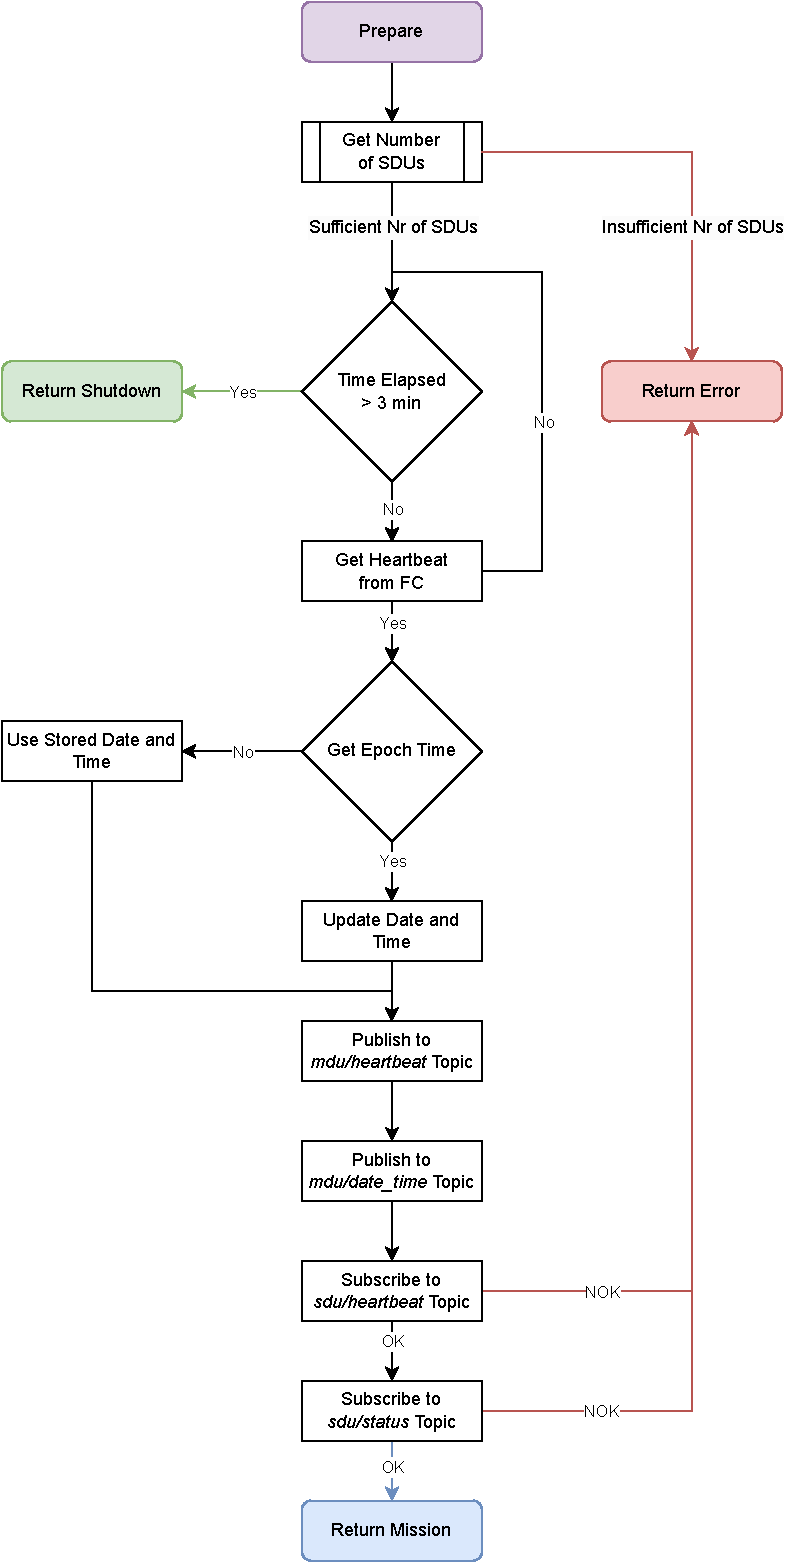
\includegraphics[scale=0.75]{appendices/assets/MDU_PREPARE.pdf}
    \caption{Proposed System Behavior - Prepare Task Flow Chart (MDU)}
    \label{fig:MDU_PREPARE}
\end{figure}

%-------------------------------------------------------------------------------%
% Appendix B

\chapter{Main Device Flow Chart - Mission Task} % Main appendix title

\label{AppendixB}

\begin{algorithm}[H]
    \centering
    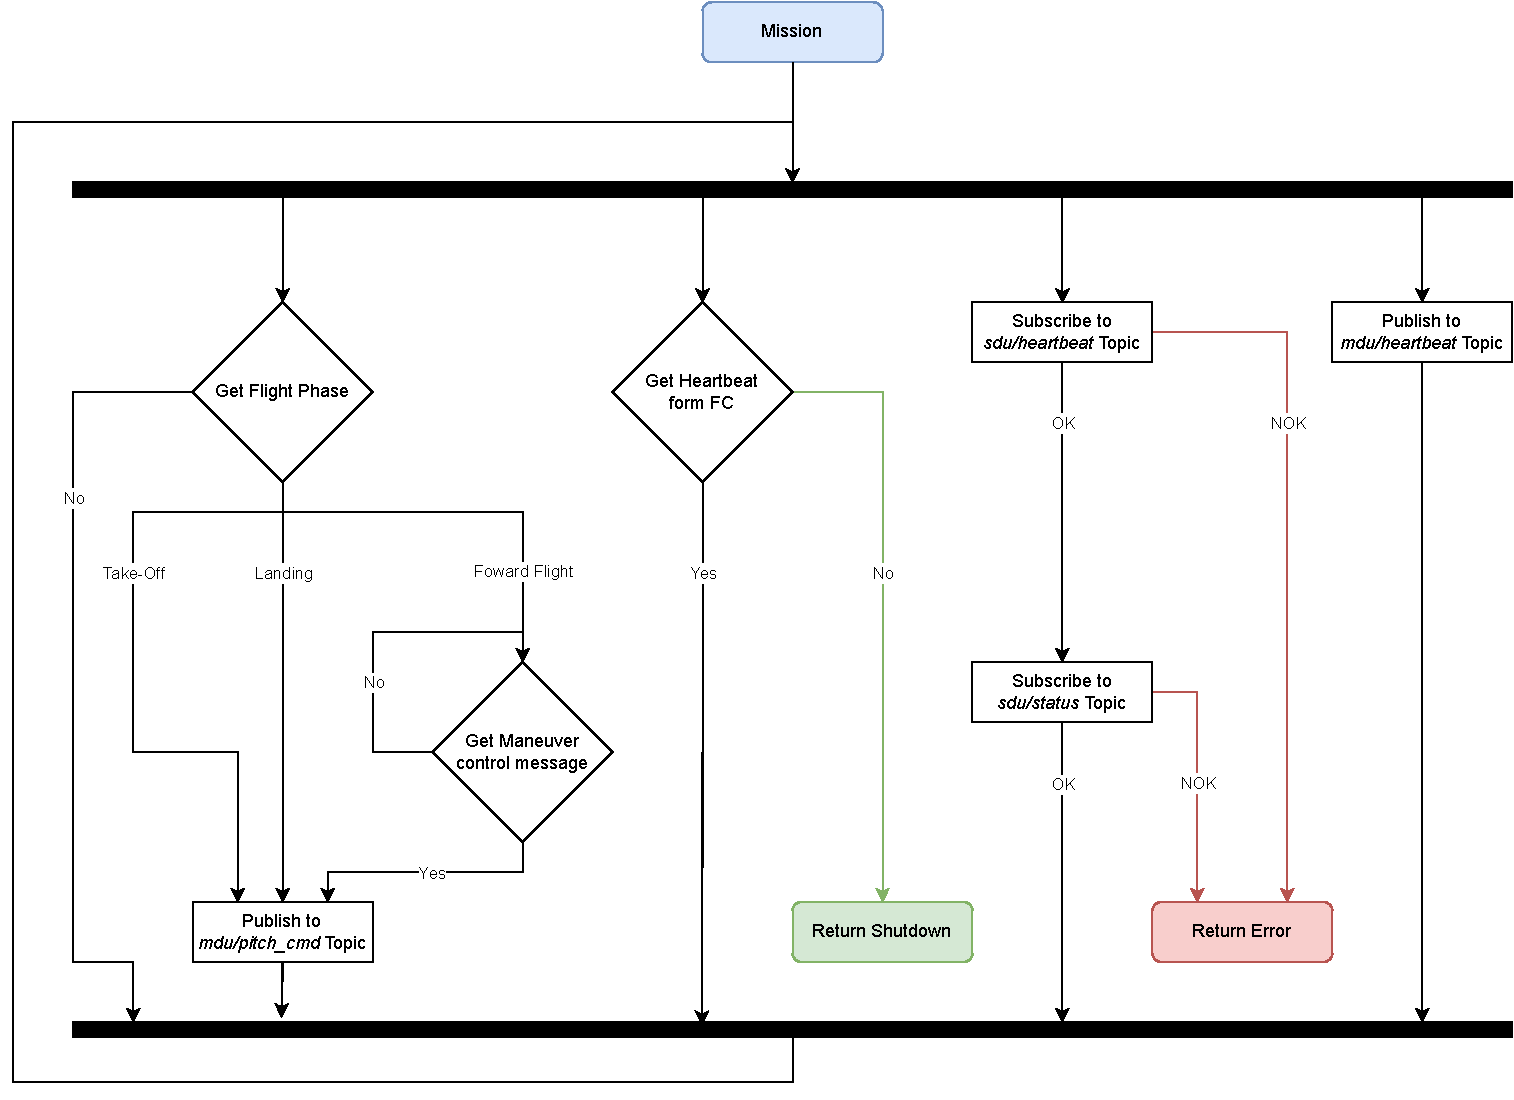
\includegraphics[scale=0.6,angle=270,origin=c]{appendices/assets/MDU_MISSION.pdf}
    \caption{Proposed System Behavior - Mission Task Flow Chart (MDU)}
    \label{alg:MDU_MISSION}
\end{algorithm}

%-------------------------------------------------------------------------------%
% Appendix C

\chapter{Main Device Flow Chart - Error Task} % Main appendix title

\label{AppendixC}

\begin{algorithm}[H]
    \centering
    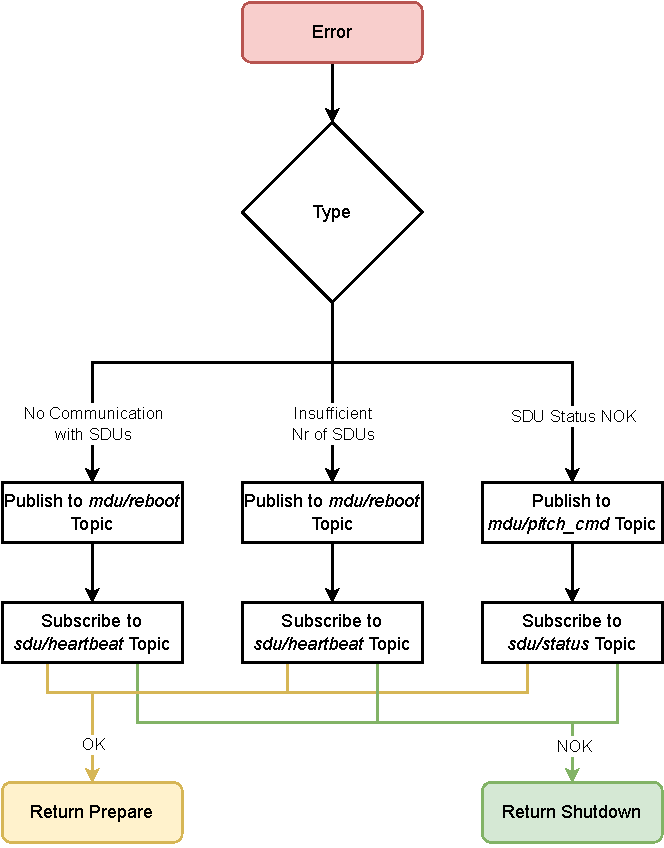
\includegraphics[scale=1]{appendices/assets/MDU_ERROR.pdf}
    \caption{Proposed System Behavior - Error Task Flow Chart (MDU)}
    \label{alg:MDU_ERROR}
\end{algorithm}

%-------------------------------------------------------------------------------%
% Appendix D

\chapter{Main Device Flow Chart - Shutdown Task} % Main appendix title

\label{AppendixD}

\begin{figure}[H]
    \centering
    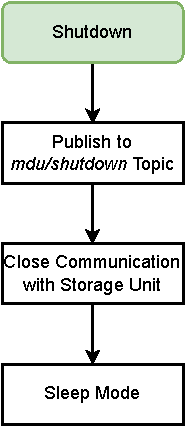
\includegraphics[scale=1]{appendices/assets/MDU_SHUTDOWN.pdf}
    \caption{Proposed System Behavior - Shutdown Task Flow Chart (MDU)}
    \label{fig:MDU_SHUTDOWN}
\end{figure}

%-------------------------------------------------------------------------------%

% Appendix E

\chapter{Secondary Devices Flow Chart - Prepare Task} % Main appendix title

\label{AppendixE}

\begin{figure}[H]
    \centering
    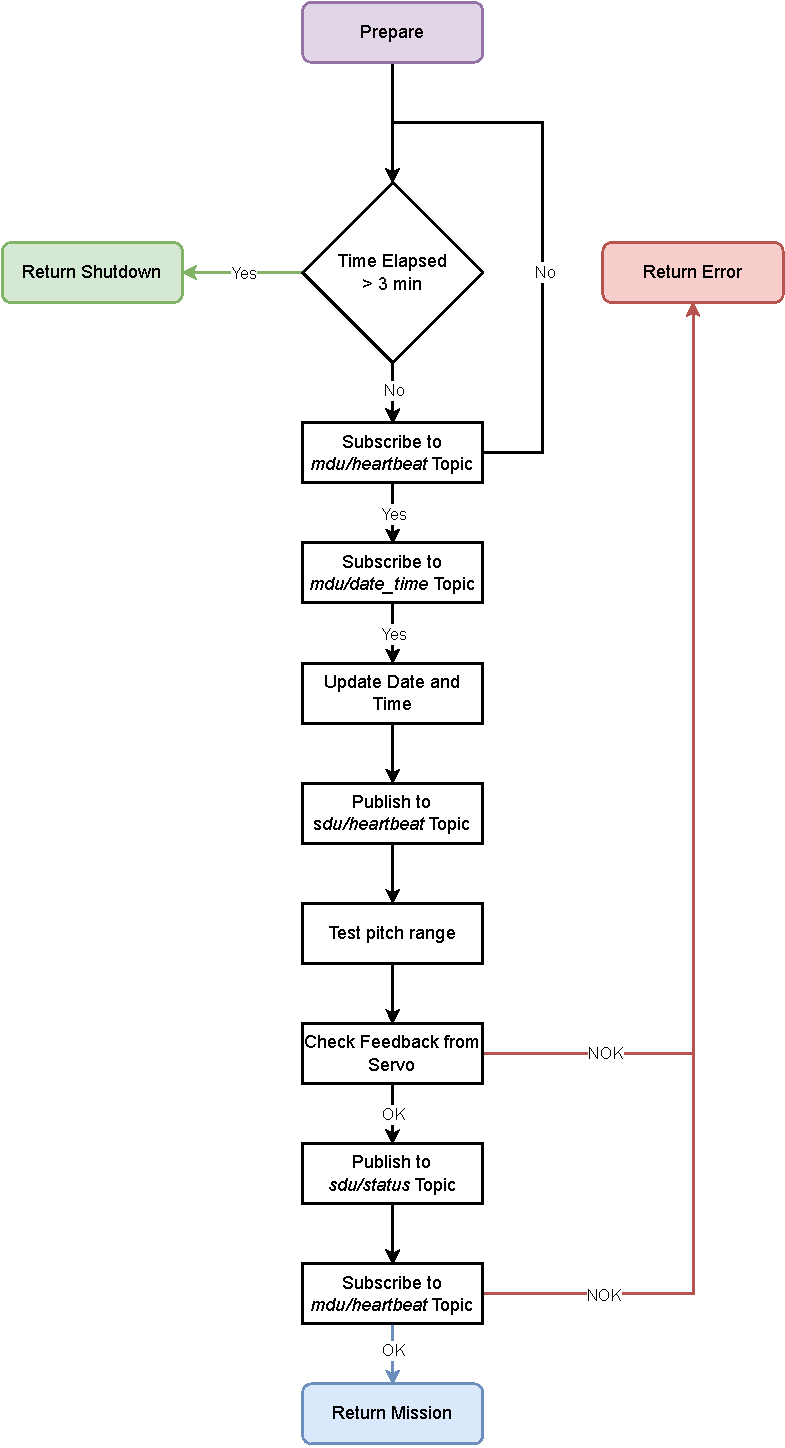
\includegraphics[scale=0.75]{appendices/assets/SDU_PREPARE.pdf}
    \caption{Proposed System Behavior - Prepare Task Flow Chart (SDU)}
    \label{fig:SDU_PREPARE}
\end{figure}

%-------------------------------------------------------------------------------%
% Appendix F

\chapter{Secondary Devices Flow Chart - Mission Task} % Main appendix title

\label{AppendixF}

\begin{figure}[H]
    \centering
    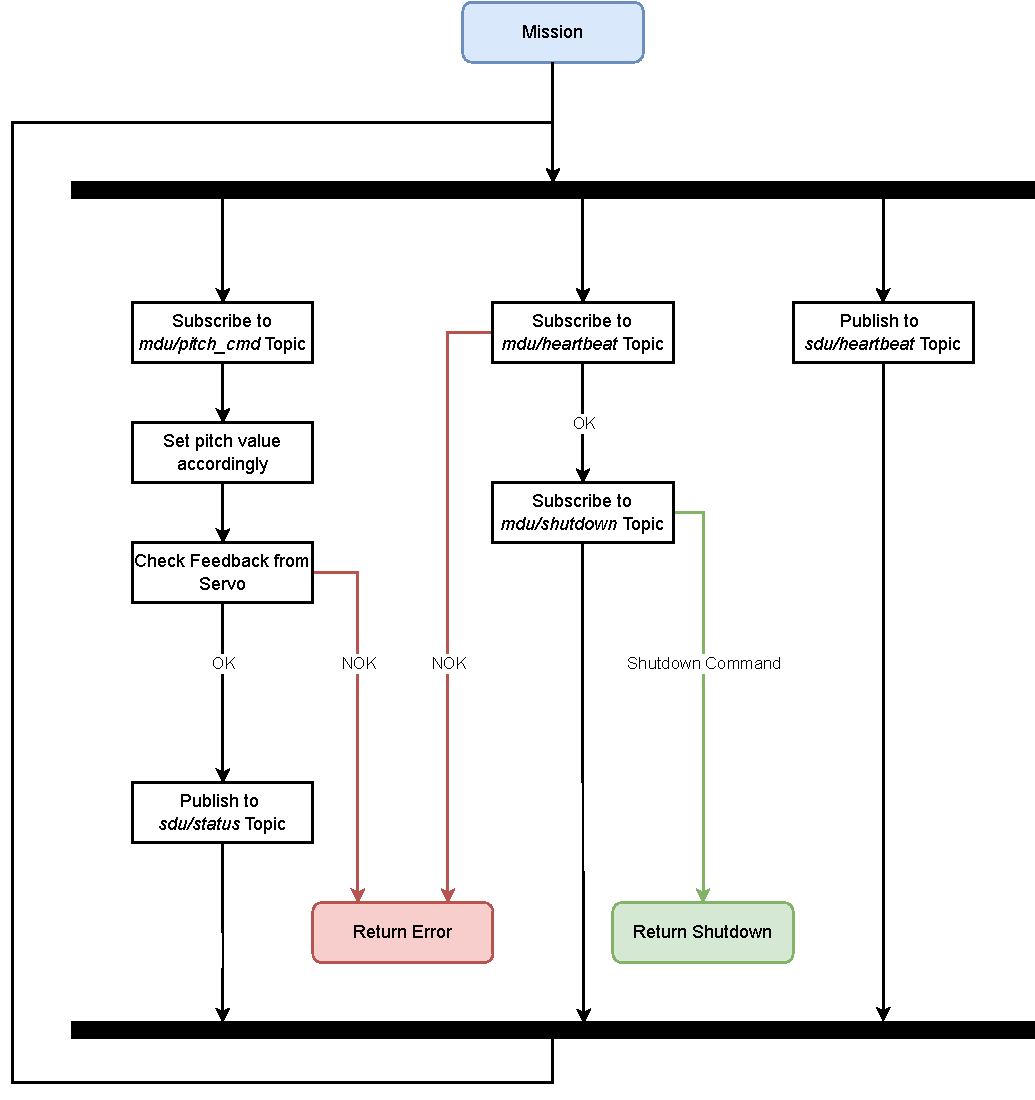
\includegraphics[scale=0.75]{appendices/assets/SDU_MISSION.pdf}
    \caption{Proposed System Behavior - Mission Task Flow Chart (SDU)}
    \label{fig:SDU_MISSION}
\end{figure}

%-------------------------------------------------------------------------------%
% Appendix G

\chapter{Secondary Devices Flow Chart - Error Task} % Main appendix title

\label{AppendixG}

\begin{figure}[H]
    \centering
    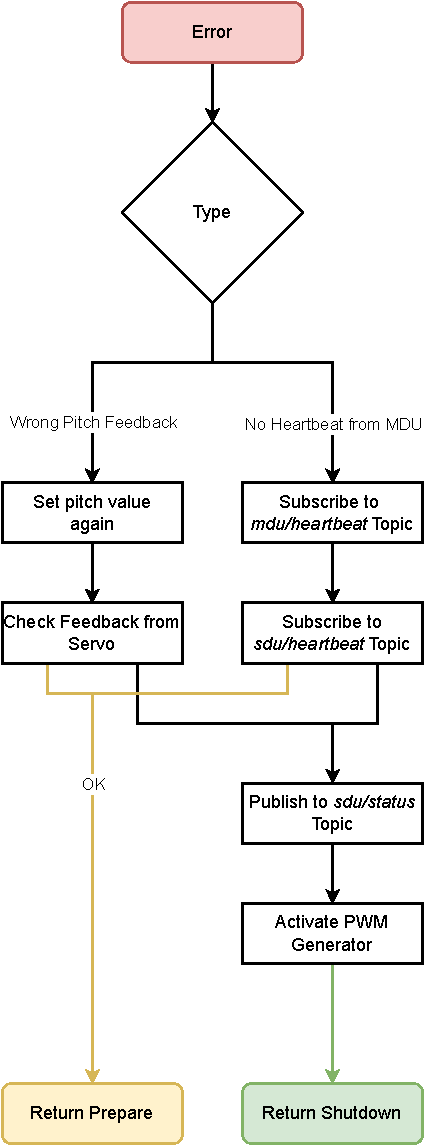
\includegraphics[scale=0.75]{appendices/assets/SDU_ERROR.pdf}
    \caption{Proposed System Behavior - Error Task Flow Chart (SDU)}
    \label{fig:SDU_ERROR}
\end{figure}

%-------------------------------------------------------------------------------%
% Appendix H

\chapter{Secondary Devices Flow Chart - Shutdown Task} % Main appendix title

\label{AppendixH}

\begin{figure}[H]
    \centering
    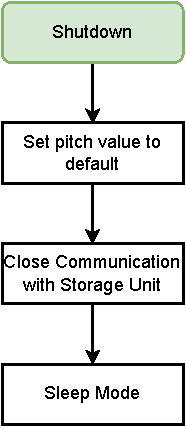
\includegraphics[scale=1]{appendices/assets/SDU_SHUTDOWN.pdf}
    \caption{Proposed System Behavior - Shutdown Task Flow Chart (SDU)}
    \label{fig:SDU_SHUTDOWN}
\end{figure}

%-------------------------------------------------------------------------------%
%----------------------------------------------------------------------------------------

\end{document}
